\begin{figure*}[t]
  \centering
  \begin{subfigure}{0pt}\phantomsubcaption\label{fig:hero-gam}\end{subfigure}%
  \begin{subfigure}{0pt}\phantomsubcaption\label{fig:hero-calm}\end{subfigure}%
  \begin{subfigure}{0pt}\phantomsubcaption\label{fig:hero-ga2m}\end{subfigure}%
  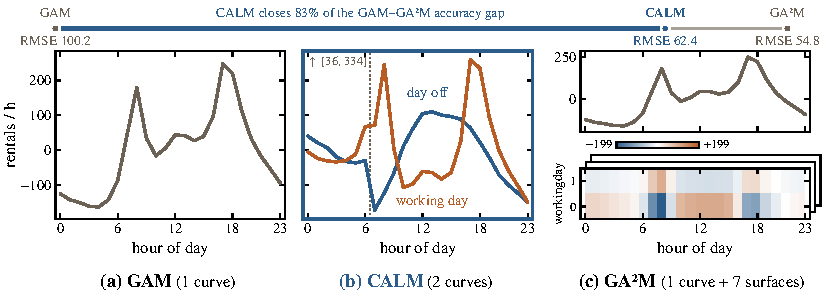
\includegraphics[width=\linewidth]{images/bike/hero}
  \caption{The effect of the hour on bike rentals (Bike Sharing dataset). Top: test RMSE (Table~\ref{tab:regr-rmse}); CALM closes 83\% of the gap from GAM to \gamm.
    (\subref{fig:hero-gam}) GAM: one curve. The interaction with the working day is averaged away, which limits accuracy.
    (\subref{fig:hero-calm}) CALM: one curve for working days and one for days off (at $d_{\max} = 1$). The dotted line mark a hidden jump (see Section~\ref{subsec:interpretability-properties} for more details).
    (\subref{fig:hero-ga2m}) \gamm: a curve and seven 2D surfaces (only one shown here) for decoding the effect of the hour, which limits its interpretability.}
  \label{fig:hero}
\end{figure*}
